\documentclass[a4paper,11pt]{jsarticle}


% 数式
\usepackage{amsmath,amsfonts}
\usepackage{bm}
% 画像
\usepackage[dvipdfmx]{graphicx}


\begin{document}

\title{勾配降下法による学習}
\author{須賀勇貴}
\date{最終更新日:\today}
\maketitle
ここでは,勾配降下法について説明する.主に瀧先生の「これならわかるディープラーニング入門」を参考にして書いた.\par
\vspace{1cm}

\section{勾配降下法}
ニューラルネットワークの学習は損失関数の最小化によって行われる.つまり,ネットワークパラメータの空間上でスカラー関数$L(\bm{\theta})$の最小値を探すという最適化問題を解くことになる.
\begin{equation}
  \bm{\theta} = \underset{\bm{\theta}} {\operatorname{argmin}} L(\bm{\theta})
\end{equation}
損失関数は基本的に多くのパラメータを含む複雑な関数であるため,このような最適化問題を厳密に解くことはできない.そのため,計算機によって数値的に近似解を求めることになる.\par

\subsection{勾配降下法}
誤差関数$E(\bm{\theta})$の最小点を見つける手法のうち,最も直観的で単純なアイデアは図\ref{gradient_decent}のように,誤差関数のグラフの形状をした凹みにおいて.上のほうからボールを転がり落してボールの一番低いところにたどり着くまで待つ方法である.これがまさに勾配降下法の考え方である.\par

\begin{figure}
  \begin{center}
    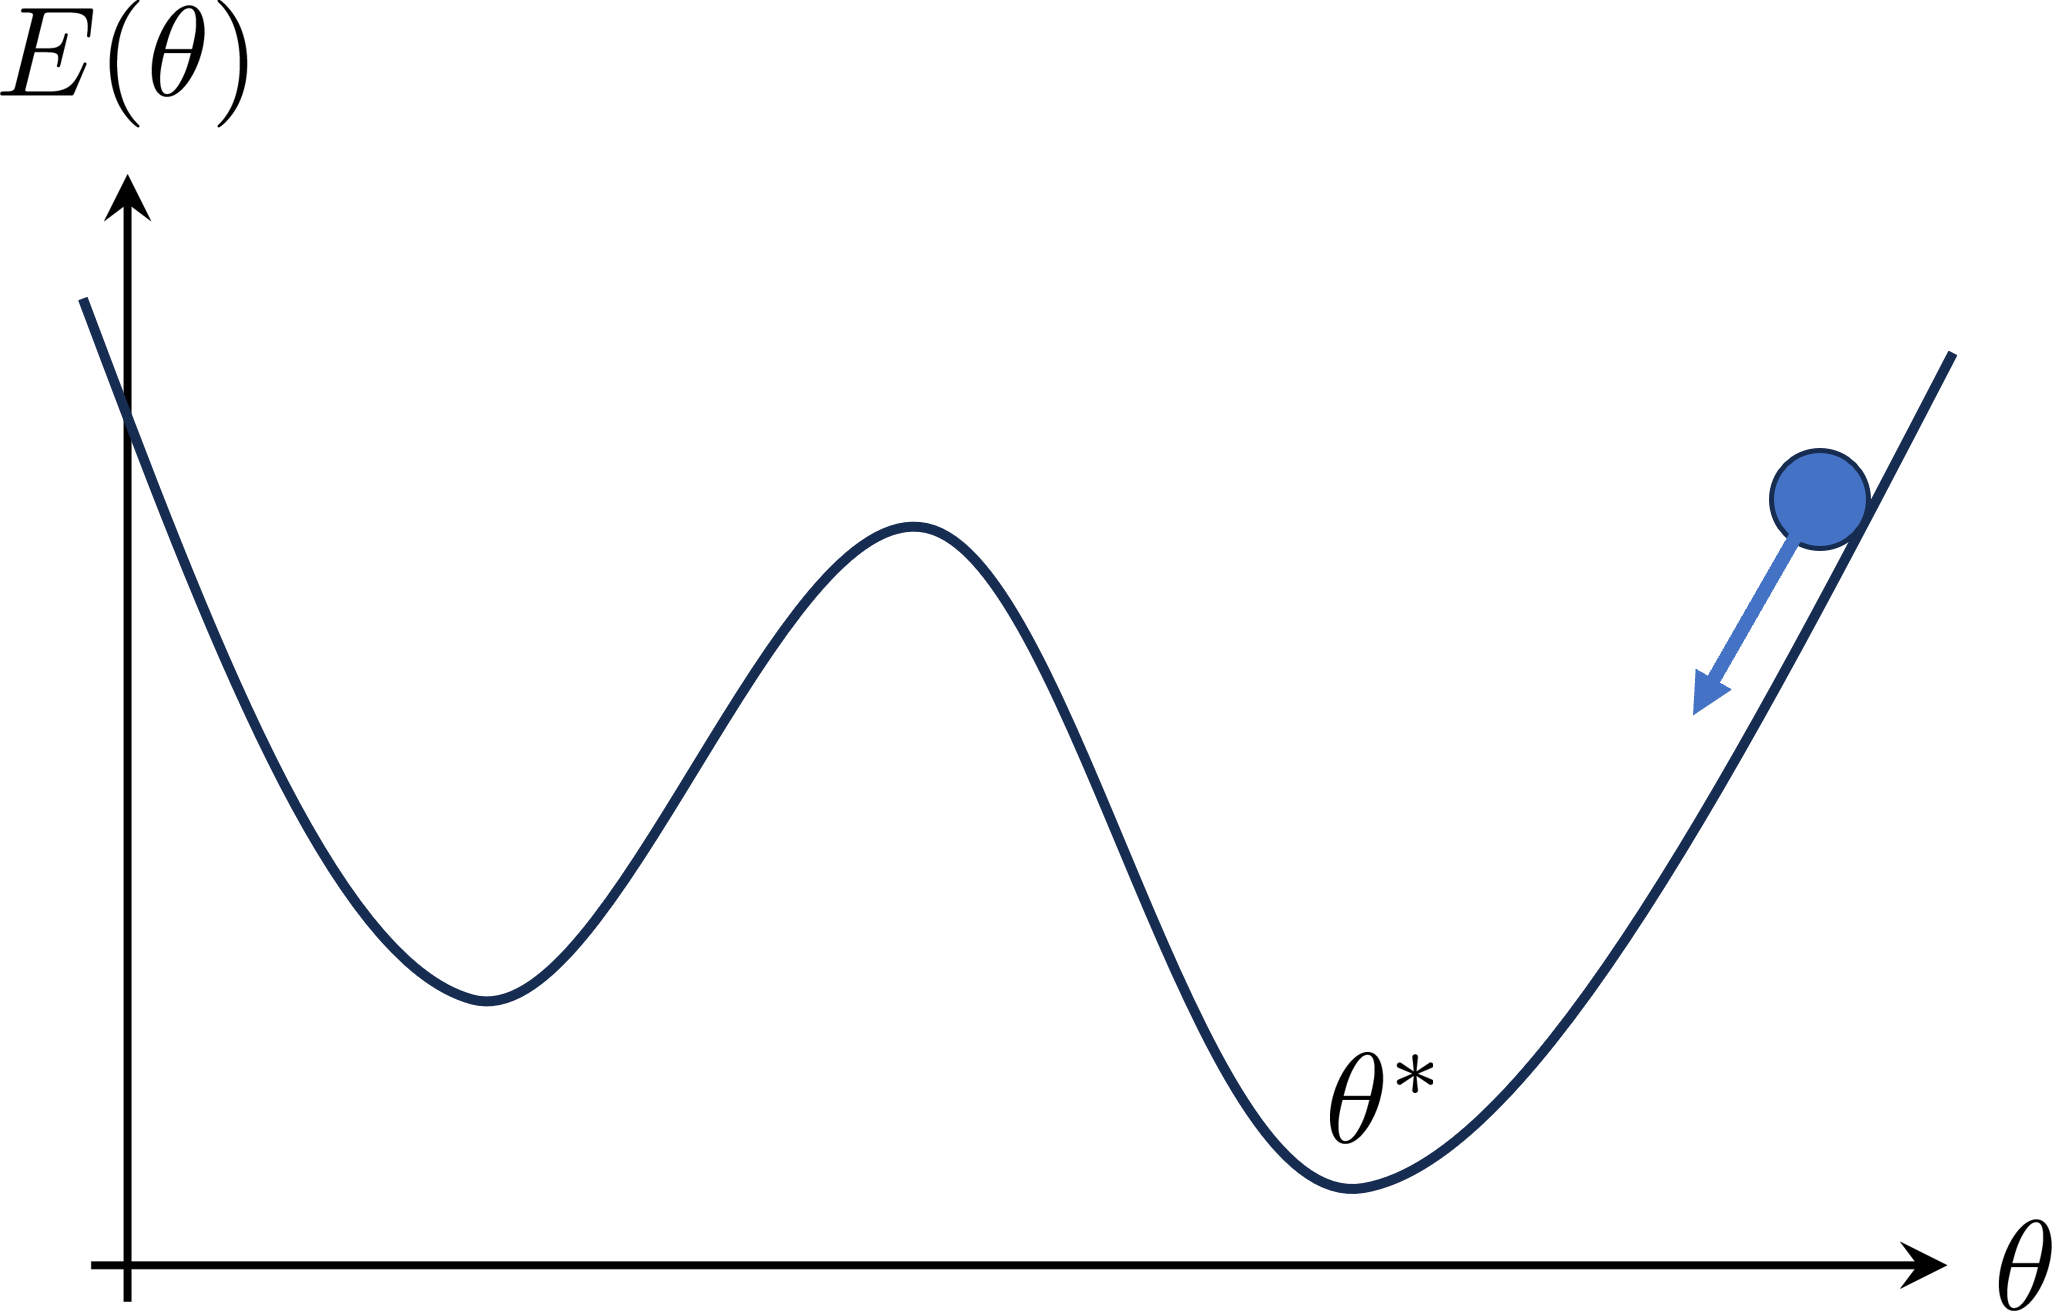
\includegraphics[height=5cm]{graph/gradient_decent.png}
    \caption{勾配降下法による極小値の見つけ方.\label{gradient_decent}}
  \end{center}
\end{figure}

ボールを転がり始めさせる位置に対応して,勾配降下法ではパラメータの初期値$\theta^{(0)}$を用意する.この初期値から始めて,坂道でボールを転がすような操作を,離散的な時間$t=0,1,2,\dots$を用いて定式化しよう.坂を転がすというのは,現在位置におけるグラフの勾配
\begin{equation}
  \nabla E(\bm{\theta})
  = \frac{\partial E(\bm{\theta})}{\partial \bm{\theta}}
  \equiv \left(  \frac{\partial E(\bm{\theta})}{\partial \theta_1}, \cdots,  \frac{\partial E(\bm{\theta})}{\partial \theta_D} \right)
\end{equation}
の逆方向に動かすことを意味する.ここで表記を簡単にするため,ニューラルネットワークの重みパラメータを下付き添え字$\theta_1,\theta_2,\dots,\theta_D$でラベル付けした.$D$はニューラルネットワークの全パラメータ数である.すると時刻$t$で位置$\bm{\theta^{(t)}}$にあったボールを勾配の逆方向に動かす際のルールは次のようになる.
\begin{equation}
  \bm{\theta^{(t+1)}} = \bm{\theta^{(t)}} + \Delta \bm{\theta^{(t)}} , \ \  \Delta \bm{\theta^{(t)}} = - \varepsilon \nabla E\left( \bm{\theta}^{(t)} \right)
\end{equation}
右辺で次時刻の$\theta^{(t+1)}$を定義する操作を$t=0,1,2,\dots$と順次繰り返していくことで,どんどんと誤差関数のグラフの底のほうに降りていくことができる.$1$ステップでの移動距離$\Delta \bm{\theta^{(t)}}$の大きさを決めるハイパーパラメータ$\varepsilon$は学習率(learning late)と呼ばれる.この操作が収束し,もはや動けなくなった点が勾配が消える極小値である.ここでいう収束とは,計算機の数値制度の範囲内でもはや$\theta^{(t)}$の変化が見られなくなる状況のことである.\par
学習率の取り方には一般論は存在せず,現状ではトライアルアンドエラーに基づかざるを得ない.しかし学習率をあまり大きくすると,$1$ステップの刻みが荒らすぎて誤差関数の形状をうまく捉えられずに,収束に問題を起こす.その一方であまり小さくしすぎると学習が一向に進まなくなる.したがって,程よい大きさの学習率を見つけることが,学習をうまく進めるために重要となる.\par

\subsection{局所的最小値の問題}
いままでは最小値と極小値の区別に注意を払わなかった.誤差関数が下に凸な関数である簡単な状況では任意の極小値は必ず最小値に一致するので区別する必要がない.しかしながらディープラーニングにおける誤差関数は一般的にとても複雑な非凸関数なので,本当の極小値である大域的極小値以外にも,膨大な数の局所的極小値をもつ.\par
さらにニューラルネットワークには高い対称性と極小値の重複がある.例えば,第$l$層の2つのユニット$j=1,2$に注目すると,この2つのユニットを入れ替えても最終層の出力は変わらない.なぜなら,$\theta_{1i}^{(l)},\theta_{k1}^{(l+1)}$と$\theta_{2i}^{(l)},\theta_{k2}^{(l+1)}$をすべて同時に入れ替えれば何もしていないことと同じになるからである.各層でこのような入れ替えは${}_{d_l} C_2$通りだけある.したがってニューラルネットワーク全体では$\prod_l {}_{d_l} C_2$通りだけの入れ替え対称性があることがわかる.つまり,局所的極小値が1つでも見つかれば,自動的に$\prod_l {}_{d_l} C_2$個の極小値が重複して存在することになる.このように,深層モデルでは極小値の数は膨大になる.\par
このような場合,勾配降下法で大域的極小値を探すのは,干草の中から針を探すようなものである.したがってディープラーニングでは極小値にはたどり着けても,真の極小値にはまずたどり着けない.通常の機械学習の文脈ではこれは深刻な問題であり,局所的最小値の問題や局所的最適解の問題と呼ばれる.\par
ところが不思議なことに,ディープラーニングでは真の最小値を見つけずとも,誤差関数のよい極小値さえ見つけられれば十分であると予想されている.これはディープラーニングを他の機械学習とは一線を画す画期的な手法にしていると同時に,ディープラーニングにおける大きな謎の1つである.この点に関しては現在でもさまざまな研究がなされている.\par

\subsection{確率的勾配降下法}
ディープラーニングが真の最小値を必要としないとはいっても,誤差関数の値があまりに大きい臨界点にはまり込んでしまっては全く使い物にならない.そこで臨界点にトラップされることをできるだけ回避するためにランダムな要素を取り入れて,はまり込んだ場所から弾き出す効果を生み出すことで勾配降下法を改良していく.\par
ランダムな要素を入れるためには,学習の仕組みを復習する必要がある.学習データ$\mathcal{D}=\{(\bm{x}_n,\bm{y}_n)\}_{n=1,2,\dots,N}$が与えられたとき,誤差関数は各学習サンプル要素$(\bm{x}_n,\bm{y}_n)$で計算した誤差の和として表現できた.
\begin{equation}
  E(\bm{\theta}) = \frac{1}{N}\sum_{n=1}^{N}E_n(\bm{\bm{\theta}}) \label{勾配降下法}
\end{equation}
例えば平均二乗誤差を用いるならば
\begin{equation}
  E_n(\bm{\bm{\theta}}) = \frac{1}{2}\left( \bm{y}(\bm{x}_n ; \bm{\theta}) - \bm{y}_n \right)^2
\end{equation}
であり,$K$クラス分類ならば交差エントロピー
\begin{equation}
  E_n(\bm{\bm{\theta}}) = - \sum_{k=1}^{K} t_{nk}\log{y_k(\bm{x}_n ; \bm{\theta})}
\end{equation}
を用いた.先ほどの勾配降下法では式(\ref{勾配降下法})のように毎回の更新ですべての訓練サンプルを用いていた.このような方法はバッチ学習と呼ばれる.\par
しかし勾配によるパラメータ更新は何回も繰り返すことになるので,1回の更新で毎回すべてのサンプルを用いる必要がない.各時間ステップで,一部の訓練サンプルだけを用いる方法をミニバッチ学習という.ミニバッチ学習ではまず,各時間$t$で用いる訓練サンプルの部分集合$\mathcal{B}^{(t)}$を用意する.この$\mathcal{B}^{(t)}$のことをミニバッチと呼び,通常は学習前にランダムに作成しておく,そして時刻$t$における更新ではミニバッチ上で平均した誤差関数
\begin{equation}
  E^{(t)}(\bm{\theta}) = \frac{1}{\mathcal{B}^{(t)}} \sum_{n\in \mathcal{B}^{(t)}} E_n(\bm{\theta})
\end{equation}
を用いる.ここで$n\in \mathcal{B}^{(t)}$はミニバッチに含まれる訓練サンプルのラベルを表し,$|\mathcal{B}^{(t)}|$はミニバッチの中のサンプル要素の総数である.これを用いてバッチ学習同様,パラメータを更新する.
\begin{equation}
  \bm{\theta^{(t+1)}} = \bm{\theta^{(t)}} + \Delta \bm{\theta^{(t)}} , \ \  \Delta \bm{\theta^{(t)}} = - \varepsilon \nabla E^{(t)}\left( \bm{\theta}^{(t)} \right)
\end{equation}
特に各時刻のミニバッチに1つの訓練サンプルしか含まない$|\mathcal{B}^{(t)}|=1$という場合をオンライン学習や確率的勾配降下法と呼ぶ.\par
ミニバッチ学習ではランダムにミニバッチを選んだことにより,時刻ごとに誤差関数$E^{(t)}(\bm{\theta})$の形もランダムに変化する.したがって,ずっと同じ関数$E(\bm{\theta})$を使い続けるバッチ学習とは違い,望ましくない臨界点にはまり込む可能性がかなり小さくなる.これがミニバッチ学習が重宝される大きな理由である.\par
さらにサンプルを効率的に使う観点からもミニバッチは好まれる.訓練データのサイズが大きくなると,似たようなサンプルが含まれる可能性が高くなる.そこで訓練データ集合全体ではなく,ミニバッチを使用することで,1回の更新ステップにおいて似たデータを重複して使用する無駄が省けるようになる.\par
またミニバッチでの勾配降下法では,各勾配$\nabla E_n(\bm{\theta})$の計算が独立で容易に並列化できる.したがって,コアのたくさんあるGPGPUなどの並列計算環境がある場合には,ある程度のサイズのミニバッチを利用するほうが理にかなっている.

\subsection{ミニバッチの作り方}
(ミニ)バッチ学習では,学習時間をエポック(epoch)という単位ごとに分けて考える.1エポックという単位は,訓練データ全体を1周すべて使い切る時間単位を意味する.\par
まずはじめのエポックでは,データを適当なサイズのミニバッチにランダムに分割する.そして,これらのミニバッチを用いて勾配を更新していく.すべてのミニバッチを使い切ったら,このエポックは終了になる.しかし通常は,1エポックでは不十分で,次のエポックに進み,改めてランダムにミニバッチを作り,同じプロセスを繰り返していく,そして,誤差関数が十分小さくなるまでエポックを繰り返したら,学習終了になる.\par
また,バッチ学習では毎回データを使い切るため,エポックと更新時間は一致する.

\subsection{収束と学習率のスケジューリング}



\end{document}